\documentclass[14pt,dvipdfmx]{beamer}
% pdfの栞の字化けを防ぐ
% \AtBeginDvi{\special{pdf:tounicode EUC-UCS2}}
% テーマ
%\usetheme{AnnArbor}
\usetheme{Madrid}
% navi. symbolsは目立たないが,dvipdfmxを使うと機能しないので非表示に
\setbeamertemplate{navigation symbols}{} 
\usepackage{graphicx}
\usepackage{amsmath}
\usepackage{amsfonts}
\usepackage{amssymb}
\usepackage{ascmac}
\usepackage{comment}
% フォントはお好みで
\usepackage{txfonts}
\usepackage{here}
\usepackage{slashbox}
\usepackage[labelformat=empty,labelsep=none]{caption}
%\mathversion{bold}
\renewcommand{\familydefault}{\sfdefault}
\renewcommand{\kanjifamilydefault}{\gtdefault}
\setbeamerfont{title}{size=\large,series=\bfseries}
\setbeamerfont{frametitle}{size=\large,series=\bfseries}
\setbeamertemplate{frametitle}[default]
\usefonttheme{professionalfonts}
\newcommand{\backupbegin}{
  \newcounter{framenumberappendix}
  \setcounter{framenumberappendix}{\value{framenumber}}
}
\newcommand{\backupend}{
  \addtocounter{framenumberappendix}{-\value{framenumber}}
  \addtocounter{framenumber}{\value{framenumberappendix}} 
}
\newcommand{\bd}[1]{\mbox{\boldmath $#1$}}
\def\smskip{\par\vskip 5pt}
\def\QED{\hfill $\Box$ \smskip}
%
\title[設置者の稼働時間を考慮した\\止水板最適設置順序の算出]{設置者の稼働時間を考慮した\\止水板最適設置順序の算出}
\institute[システム最適化研究室]{\normalsize{システム最適化研究室}}
\author{都14-86 竹内 美紗}
\date{2018/2/16}

\begin{document}
%%%%%%%%%%%%%%%%%%%%%%%%%%%%%%%%%%%%%%%%%%%%%%%%%%%%%%%%5
\frame{\titlepage}
%%%%%%%%%%%%%%%%%%%%%%%%%%%%%%%%%%%%%%%%%%%%%%%%%%%%%%%
\frame{
   \frametitle{本研究の背景 (1/2)}
   \vspace{-5mm}

  \begin{beamerboxesrounded}
    {豪雨の事例 : 福岡豪雨 (1999)}
      \small
      \begin{itemize}
      \item 6 月 29 日発生
      \item 1 時間最大雨量 79.5mm
      \item ビル 182 棟のうち 71 棟の地下が浸水,死者 37 名
      \end{itemize}
  \end{beamerboxesrounded}
  \begin{beamerboxesrounded}
    {先行研究}
    \begin{itemize}
      \small
    \item 森兼ら(2011)によって地下空間に流入する出入口の場所,流入順序,流入時間,流入量を推定できることが分かった
    \item 武田の研究(2015)ではホワイティうめだを対象として内水氾濫シュミレーションにより止水板の設置順序やタイミングを検討
    \item 馬谷の研究(2016)では梅田地下街全域を対象とし,最適化問題としてソルバで最適設置順序を算出
    \end{itemize}
  \end{beamerboxesrounded}

  

    
}
%%%%%%%%%%%%%%%%%%%%%%%%%%%%%%%%%%%%%%%%%%%%%%%%%%%%%%%%%
%% \frame{
%%   \frametitle{本研究の背景 (2/2)}
%%   \vspace{-4mm}
%%   \begin{beamerboxesrounded}
%%     {先行研究}
%%     \begin{itemize}
%%       \small
%%     \item 地下空間に流入する出入口の場所,流入順序,流入時間,流入量を推定することができる\\
%%       $\Rightarrow$ 事前に止水活動や避難誘導が可能である\\
%%       \vspace{3mm}
%%     \item ホワイティうめだを対象として内水氾濫シュミレーションにより止水板の設置順序やタイミングを検討\\
%%       $\Rightarrow$ 最適な設置順序であるか検討が不十分\\
%%       \vspace{3mm}
%%     \item 梅田地下街全域を対象として最適化問題としてソルバで最適設置順序を算出\\
%%       $\Rightarrow$ 梅田の管理主体を考慮できていない\\
%%       $\Rightarrow$ 設置チームの稼働時間の考慮ができていないため負荷が大きい
%%     \end{itemize}
%%   \end{beamerboxesrounded}

%% }
%%%%%%%%%%%%%%%%%%%%%%%%%%%%%%%%%%%%%%%%%%%%%%%%%%%%%%%
\frame{
  \frametitle{本研究の目的}

  \begin{beamerboxesrounded}
    {課題}
    \begin{itemize}
    \item 止水板設置に要する負荷は大きいものであるため稼働時間には限界がある
    \item 梅田地下街には複数の管理主体が存在する
    \end{itemize}
  \end{beamerboxesrounded}
    \vspace{4mm}
  \begin{beamerboxesrounded}
    {目的}
    \begin{itemize}
    \item 設置チームの稼働時間を制限して設置可能であるかを検討
    \item 梅田地下街の管理主体を考慮した止水板設置順序の算出
    \end{itemize}
  \end{beamerboxesrounded}

}
%%%%%%%%%%%%%%%%%%%%%%%%%%%%%%%%%%%%%%%%%%%%%%%%%%%%%%%
%% \frame{
%%   \frametitle{本研究に現れる時空間ネットワーク}
%%   \vspace{-4mm}
%%   \begin{figure}[H]
%%     \centering
%%     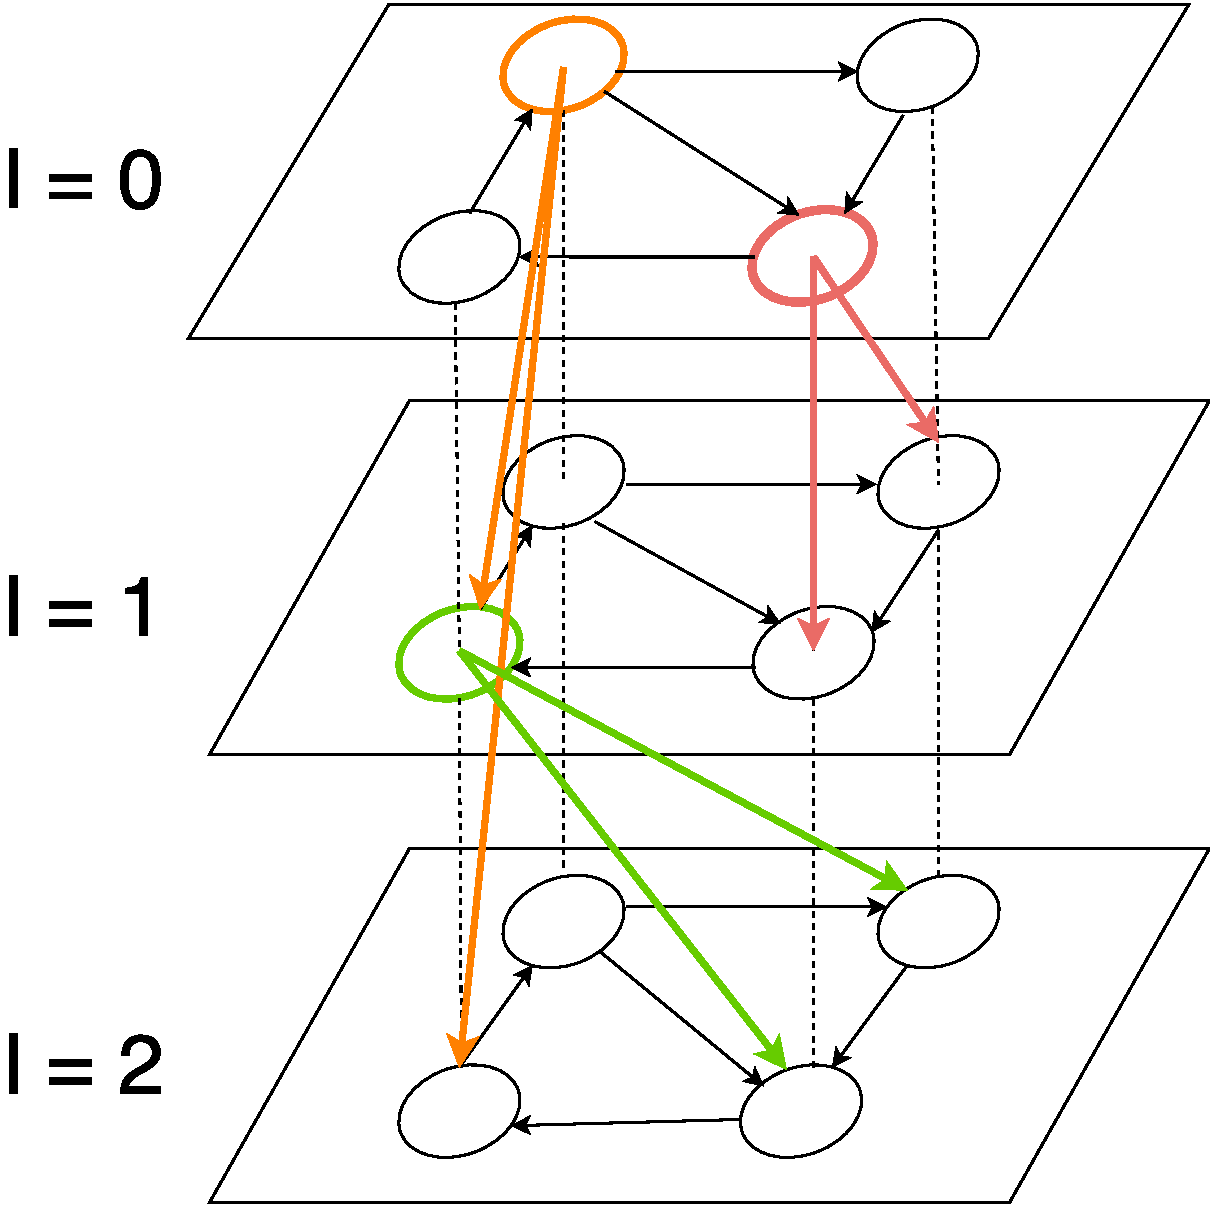
\includegraphics[width=59mm]{nettowaku.pdf}
%%     \vspace{-4mm}
%%     \label{時空間ネットワーク}
%%   \end{figure}
%%   \begin{itemize}
%%   \item 各チームの移動回数を $l= 0, 1, 2...$ とし,レイヤに対応させる
%%   \item 場所と時間が同時に表現できる
%%   \end{itemize}

%% }

%%%%%%%%%%%%%%%%%%%%%%%%%%%%%%%%%%%%%%%%%%%%%%%%%%%%%%%
%% \frame{
%%   \frametitle{本研究で用いる最適化問題}
%%   本研究では,馬谷の研究で提案された問題に一部修正,追加を行ったものである.
%%   \vspace{3mm}

  
%% }

%%%%%%%%%%%%%%%%%%%%%%%%%%%%%%%%%%%%%%%%%%%%%%%%%%%%%%%%
\frame{
  \frametitle{最適化問題の定式化}
%  \begin{description}
      \begin{itembox}[l]{目的関数}
        「流入開始時刻に間に合わなかった出入り口の止水板設置完了時刻」と「流入開始時刻」の差の合計を最小化
        \end{itembox}
   %% \item [制約条件 1]設置チームは定められたスタート地点に位置する
   %% \item [制約条件 2]全出入り口に止水板を設置する
   %% \item [制約条件 3]設置チームはそれぞれの移動の際に\\高々 1 つの出入り口に位置することができる
   %% \item [制約条件 4] 1 つの出入り口に移動するのは 1 チームのみである
    %% \item [制約条件 5~7]時空間ネットワークにおける枝と接点の関係性
      \begin{itembox}[l]{\textcolor{red}{修正した}制約条件}
        各出入り口の止水板設置完了時刻の計算
      \end{itembox}
%% \item [制約条件 9]流入開始するまでの時間の設定
     %% \item [制約条件 10]止水板設置完了時刻と流入開始時刻の差の計算
      \begin{itembox}[l]{\textcolor{red}{追加した}制約条件}
        各設置チームの稼働時間の制限
      \end{itembox}
%\end{description}

   %\vspace{2mm}
   
 %%   \begin{itemize}
 %%   \footnotesize
 %% \item \textcolor{red}{赤色} : 修正,追加した制約条件
 %% \item \textcolor{blue}{青色} : 先行研究で提案されていた制約条件
 %%   \end{itemize}
   
%%      \begin{table}[H]
%%     \footnotesize
%%   \begin{center}
%%     %\caption{制約条件の訂正と追加}
%%     \scalebox{0.8}{
%%       \begin{tabular}{ll}\hline
%%         \vspace{3mm}
%%       馬谷の研究で提案された制約 & 制約条件 1~7, 9, 10  \\
%%       \vspace{3mm}
%%       馬谷の研究で提案された制約を修正 & 制約条件 8  \\
%%       %\vspace{3mm}
%%       新たに追加する制約 & 制約条件 11  \\\hline
%%     \end{tabular} }
%%     \label{制約条件表}
%%   \end{center}
%% \end{table}

}

%%%%%%%%%%%%%%%%%%%%%%%%%%%%%%%%%%%%%%%%%%%%%%%%%%%%%%%%
\frame{
  \frametitle{実験条件}
  \begin{table}[H]
    \begin{center}
      \begin{tabular}{ll}\hline
        計算対象域 & ホワイティうめだ\\
        1 時間当たりの降雨量 & 120mm\\
        排水用ポンプ & 稼働状態\\
        雨水が流入する出入口 & 21 箇所\\
        止水板設置チームの歩行速度 & 66m/分\\
        止水板 1 箇所の設置に要する時間 & 5 分\\
        計算時間 & 3600 秒 (= 1 時間)\\\hline
      \end{tabular}
      \label{基本条件}
    \end{center}
  \end{table}
  設置開始時刻
\begin{itemize}
\item 43 分 : 水位計より判断
\item 57 分 : 地上監視カメラより判断
\item 64 分 : 地下への流入が始まった
\end{itemize}


}
%%%%%%%%%%%%%%%%%%%%%%%%%%%%%%%%%%%%%%%%%%%%%%%%%%%%%%%
\frame{
  \frametitle{実験 1}
  止水板設置チームの稼働時間に上限がある状況下で,止水板設置に必要なチーム数の算出
  \vspace{5mm}

  \begin{itemize}
  \item 止水板設置開始時刻 : 64 分
  \end{itemize}
  
  \begin{table}[htpb]
 \begin{center}
  \caption{止水板の設置可能性}
  \scalebox{0.8}{
    \begin{tabular}{c|cccc}\hline
      \backslashbox{チーム数}{稼働時間} & 30 & 40 & 50 & 60\\\hline
   6 & 可能 & 可能 & 可能 & 可能\\
   5 & 暫定解なし & 可能 & 可能 & 可能\\
   4 & 不可能 & 可能 & 可能 & 可能\\
   3 & 不可能 & 不可能 & 暫定解なし & 可能\\
   2 & 不可能 & 不可能 & 不可能 & 不可能\\\hline
  \end{tabular}
  }
  \label{64分制限時間変化}
 \end{center}
  \end{table}

  \footnotesize
  「暫定解なし」は,設置が可能であるかどうかが判断できないことを表す.

}


%%%%%%%%%%%%%%%%%%%%%%%%%%%%%%%%%%%%%%%%%%%%%%%%%%%%%%%
\frame{
  \frametitle{実験 2 (1/2)}
  設置開始時刻による流入時間の合計の差を算出
  \vspace{5mm}

  \begin{itemize}
  \item 設置チーム数 : 6 チーム
  \item 稼働時間の上限 : 30 分
  \end{itemize}

  \begin{table}[htpb]
  \begin{center}
   \caption{設置開始時刻と流入時間の合計の関係}
   \begin{tabular}{cc}\hline
     設置開始時刻(分) & 流入時間の合計 (分) \\
     \hline
     43 & 0.00 \\
     57 & 6.03 \\
     64 & 13.91 \\
     \hline
   \end{tabular}
   \label{tb:ex2}
  \end{center}
\end{table}



}

%%%%%%%%%%%%%%%%%%%%%%%%%%%%%%%%%%%%%%%%%%%%%%%%%%%%%%%%
\frame{
  \frametitle{実験 2 (2/2)}

  \begin{figure}[tpb]
    \begin{center}
      \includegraphics[scale=0.7]<1>{st43-t6.pdf}
      \includegraphics[scale=0.6]<2>{st57-t6.pdf}
      \includegraphics[scale=0.6]<3>{st64-t6.pdf}
    \end{center}
  \end{figure}
}

%%%%%%%%%%%%%%%%%%%%%%%%%%%%%%%%%%%%%%%%%%%%%%%%%%%%%%%%
\frame{
  \frametitle{実験 3}
  稼働時間の上限がない場合の流入時間の合計を算出
  \vspace{5mm}

  \begin{itemize}
  \item 稼働時間の上限 : なし
  \end{itemize}

  \begin{table}
 \begin{center}
   \caption{チーム数・設置開始時刻と流入時間の合計の関係}
     \scalebox{0.8}{
  \begin{tabular}{c|ccc}
   \hline
   \backslashbox{($A$)}{($B$)} & 43 & 57 & 64 \\\hline
   6 & 0.00  & 6.03   & 13.91 \\
   5 & 0.00  & 6.03   & 13.91 \\
   4 & 0.00  & 6.03   & \textcolor{red}{24.21} \\
   3 & 0.00  & \textcolor{red}{34.73}  & 138.82 \\
   2 & 66.76 & 203.70 & 288.33 \\
   \hline
  \end{tabular} }
  \label{tb:ex3}
 \end{center}
  \end{table}
  \centering
 % \footnotesize

  ($A$) : 設置チーム数\\
  ($B$) : 止水板設置開始時刻(分)
  
}

%%%%%%%%%%%%%%%%%%%%%%%%%%%%%%%%%%%%%%%%%%%%%%%%%%%%%%%
%% \frame{
%%   \frametitle{実験まとめ}

%%   \begin{itemize}
%%     \item 6 チームでは制限時間 30 分の場合であっても\\全ての止水板設置可能である
%%     \vspace{3mm}
%%   \item 稼働時間を制限すると2, 3 チームでは全ての\\止水板を設置することはできない
%%      \vspace{3mm}
%%    \item 設置開始時刻が遅くなると流入時間は長くなる
%%       \vspace{3mm}
%%   \item どの設置開始時刻の場合でも,一定の設置チーム数が必要である
%%   \end{itemize}

%% }

%%%%%%%%%%%%%%%%%%%%%%%%%%%%%%%%%%%%%%%%%%%%%%%%%%%%%%%
\frame{
  \frametitle{おわりに}
  \vspace{3mm}

  \begin{beamerboxesrounded}
    {まとめ}
    \begin{itemize}
    \item 設置チームの稼働時間と管理主体を考慮して\\実験を行うことができた
    \item 多くのケースの実験を行うことができその結果を\\比較することができた
    \end{itemize}
  \end{beamerboxesrounded}

  \vspace{3mm}

  \begin{beamerboxesrounded}
    {今後の課題}
    \begin{itemize}
    \item 梅田地下街全域を対象として検討する必要がある
    \item 降雨量の変化,排水用ポンプの停止時など\\異なった条件での実験を行う必要がある
    \end{itemize}
  \end{beamerboxesrounded}
}

%%%%%%%%%%%%%%%%%%%%%%%%%%%%%%%%%%%%%%%%%%%%%%%%%%%%%%%
\appendix
\backupbegin

\frame{
  \frametitle{最適化問題の定式化}
  \footnotesize
   \begin{description}
   \item [目的関数]「流入開始時刻に間に合わなかった出入り口の止水板設置完了時刻」と「流入開始時刻」の差の合計を最小化
   \item [制約条件 1]設置チームは定められたスタート地点に位置する
   \item [制約条件 2]全出入り口に止水板を設置する
   \item [制約条件 3]設置チームはそれぞれの移動の際に\\高々 1 つの出入り口に位置することができる
   \item [制約条件 4] 1 つの出入り口に移動するのは 1 チームのみである
   \item [制約条件 5~7]時空間ネットワークにおける枝と接点の関係性
   \item [\textcolor{red}{制約条件 8}]各出入り口の止水板設置完了時刻の計算
   \item [制約条件 9]流入開始するまでの時間の設定
   \item [制約条件 10]止水板設置完了時刻と流入開始時刻の差の計算
   \item [\textcolor{red}{制約条件 11}]各設置チームの稼働時間の制限
   \end{description}
}


\frame{
  \footnotesize

  \begin{description}
    \item[\textcolor{red}{制約条件 8} : 修正前]
  \begin{equation}
    t_{l,p}=\displaystyle\sum_{l_ \in L,(v_1,v_2)\in E,\bar{l} < l}y_{v_1,v_2,l,p}w_{v_1,v_2}/66.0+lu
    \quad (l \in L,p \in P,l \geq 1)
  \end{equation}

  \bigskip

  \item[\textcolor{red}{制約条件 8} : 修正後]
  \begin{equation}
      t_{l,p}=\displaystyle\sum_{l \in L,(v_1,v_2) \in E,\bar{l} < l}y_{v_1,v_2,l,p}w_{v_1,v_2}/66.0 + u \displaystyle\sum_{v \in V,l \in L,l \geq L,l \leq 1}x_{v,l,p}
    \quad (l \in L,p \in P,l \leq L)
  \end{equation}

\bigskip
  
  \item[\textcolor{red}{制約条件 11}]
      \begin{equation}
      t_{l_{m},p} \leq T \quad (p \in P)
      \label{eq:Timelimit}
      \end{equation}
      \end{description}
}


\frame{
\begin{table}[H]
\begin{center}
\label{tb:experiment_summary}
\scalebox{0.5}{
 \begin{tabular}{ccc|r|rr}\hline
  設置開始時刻(分) & 設置チーム数 & 稼働時間上限(分) & 流入時間合計(分) & 計算時間(秒) & GAP(\%) \\ \hline
  43 & 2 & 設定なし & 66.76  & 3600.06 & 100.00 \\ \hline
  43 & 3 & 設定なし & 0.00   & 3186.69 & -- \\ \hline
  43 & 4 & 設定なし & 0.00   & 4.64    & -- \\ \hline
  43 & 5 & 設定なし & 0.00   & 402.29  & -- \\ \hline
  43 & 6 & 30       & 0.00   & 31.45   & -- \\ \hline
  43 & 6 & 設定なし & 0.00   & 230.62  & -- \\ \hline
   \end{tabular}
}
\end{center}
\end{table}
\begin{table}
\begin{center}
\label{tb:experiment_summary}
\scalebox{0.5}{
 \begin{tabular}{ccc|r|rr}\hline
  設置開始時刻(分) & 設置チーム数 & 稼働時間上限(分) & 流入時間合計(分) & 計算時間(秒) & GAP(\%) \\ \hline
  57 & 2 & 設定なし & 203.70 & 3600.28 & 100.00 \\ \hline
  57 & 3 & 設定なし & 34.73  & 3600.08 & 100.00 \\ \hline
  57 & 4 & 40       & 6.03   & 539.69  & -- \\ \hline
  57 & 4 & 設定なし & 6.03   & 427.98  & -- \\ \hline
  57 & 5 & 40       & 6.03   & 171.66  & -- \\ \hline
  57 & 5 & 設定なし & 6.03   & 89.58   & -- \\ \hline
  57 & 6 & 30       & 6.03   & 409.37  & -- \\ \hline
  57 & 6 & 設定なし & 6.03   & 59.94   & -- \\ \hline
     \end{tabular}
}
\end{center}
\end{table}
\begin{table}
\begin{center}
\label{tb:experiment_summary}
\scalebox{0.5}{
  \begin{tabular}{ccc|r|rr}\hline
  設置開始時刻(分) & 設置チーム数 & 稼働時間上限(分) & 流入時間合計(分) & 計算時間(秒) & GAP(\%) \\ \hline
  64 & 2 & 設定なし & 288.33 & 3600.09 & -- \\ \hline
  64 & 3 & 40       & 183.30 & 3600.08 & 96.84 \\ \hline
  64 & 3 & 50       & 160.09 & 3600.35 & 96.88 \\ \hline
  64 & 3 & 設定なし & 138.82 & 3600.14 & 96.40 \\ \hline
  64 & 4 & 40       & 32.45  & 3600.08 & 59.85 \\ \hline
  64 & 4 & 設定なし & 24.21  & 3600.03 & 46.18 \\ \hline
  64 & 5 & 40       & 13.91  & 1300.32 & -- \\ \hline
  64 & 5 & 設定なし & 13.91  & 939.54  & -- \\ \hline
  64 & 6 & 30       & 13.91  & 1540.24 & -- \\ \hline
  64 & 6 & 設定なし & 13.91  & 588.00  & -- \\ \hline
 \end{tabular}
}
\end{center}
\end{table}
}
    %% \vspace{2mm}
%% 設置開始 64 分,6 チーム,稼働時間制限なし
%% \begin{figure}
%%   \centering
%%   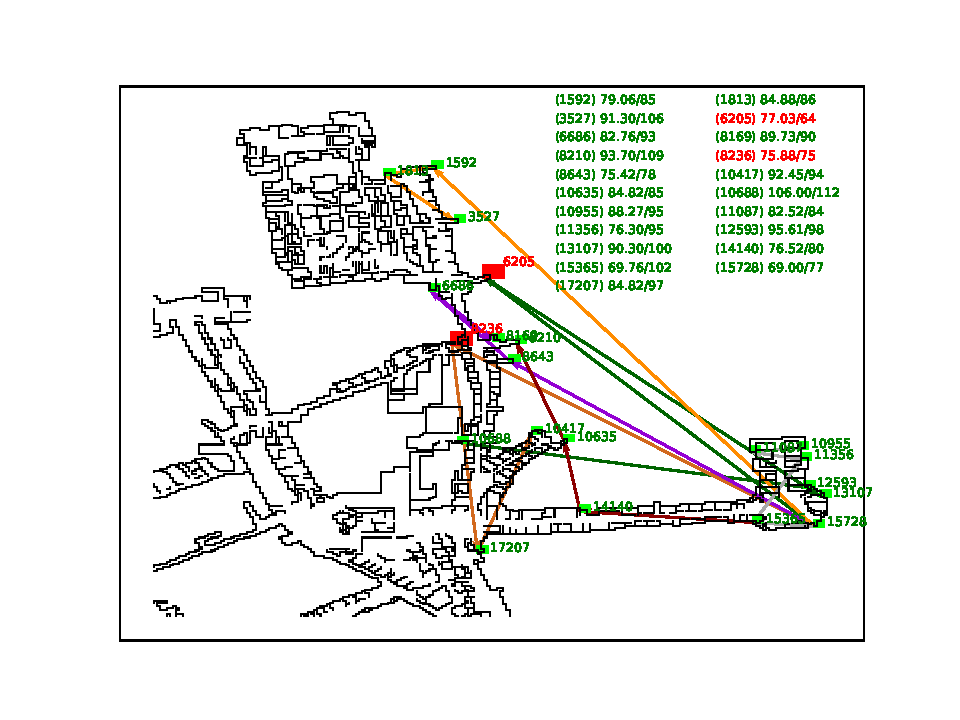
\includegraphics[scale=0.6]{st64-t6-no30.pdf}
%% \end{figure}

%% %%%%%%%%%%%%%%%%%%%%%%%%%%%%%%%%%%%%%%%%%%%%%%%%%%%%%%%%%
%% \newpage
%% 設置開始 64 分,5 チーム,稼働時間制限なし
%% \begin{figure}
%%   \centering
%%   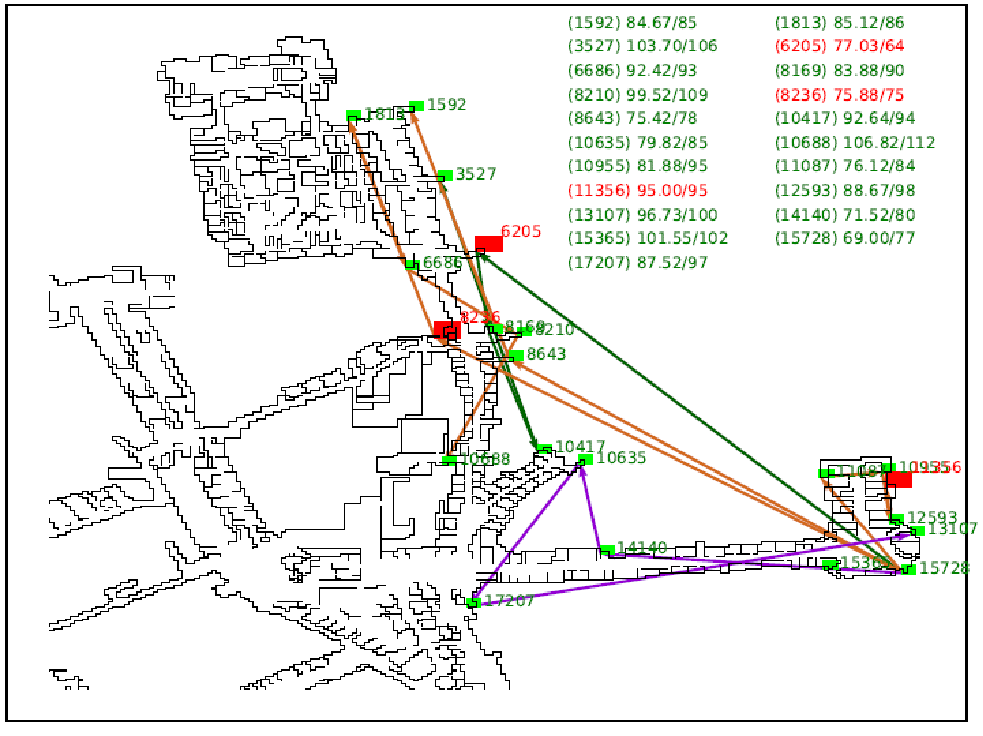
\includegraphics[scale=0.6]{st64-t5-no30.pdf}
%% \end{figure}
%% %%%%%%%%%%%%%%%%%%%%%%%%%%%%%%%%%%%%%%%%%%%%%%%%%%%%%%%%

%% \newpage
%% 設置開始 64 分,4 チーム,稼働時間制限なし
%% \begin{figure}
%%   \centering
%%   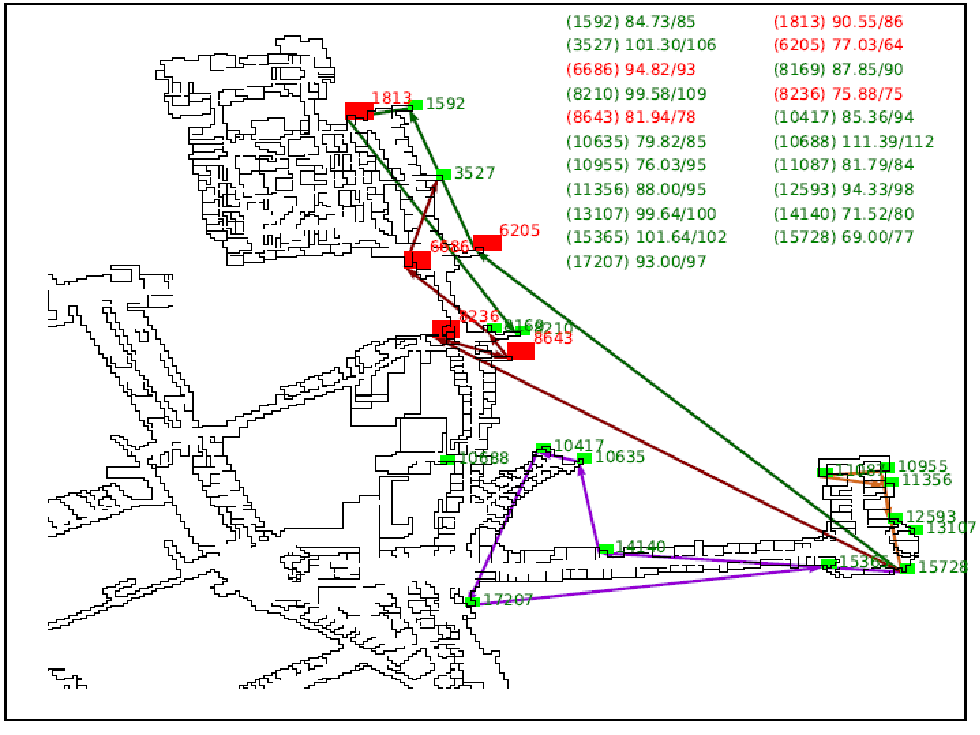
\includegraphics[scale=0.6]{st64-t4-no30.pdf}
%% \end{figure}

%% %%%%%%%%%%%%%%%%%%%%%%%%%%%%%%%%%%%%%%%%%%%%%%%%%%%%%%%%%
%% \newpage

\backupend
%%%%%%%%%%%%%%%%%%%%%%%%%%%%%%%%%%%%%%%%%%%%%%%%%%%%%%%%

\end{document}




    
